%% ma: L12-B05-0026
%% lop: 12
%% chuong: 1
%% bai: 5
%% dang: 12.5.8
%% loai: TLN
%% muc: VDC
%% dap_an: "156"
%% nguon: "(NBV)-ĐỀ SỐ 15-MỖI NGÀY 1 ĐỀ THI 2025.pdf (D15, MỖI NGÀY 1 ĐỀ - Đề số 15), Phần III Câu 5"
%% kien_thuc: "Bài 5 (tối ưu hóa bằng đạo hàm: tổng hai căn thức), Bài 1-2 (khảo sát hàm số trên đoạn)"
%% trang_thai: cho-duyet
%% ly_do: "Đề gốc thiếu giá trị vận tốc trong khu vực PMNQ (chỉ ghi chữ vận tốc, không có số). Đã bổ sung 30 km/h theo lời giải gốc; giáo viên xác nhận."
%% ghi_chu: "Đáp án gốc 156 đúng với vận tốc 30 km/h (kiểm bằng scipy: x = 35,70, 155,60 phút). Đề gốc bị thiếu số liệu vận tốc ở khu vực PMNQ; lời giải gốc dùng 30 km/h. Hình dựng lại: hình chữ nhật 50 x 40 với đường gấp khúc PXR, X thuộc MN."
\begin{ex}
Một khu rừng phòng hộ hình chữ nhật $PQRS$ có chiều dài $PQ=50\ \mathrm{km}$, chiều rộng $PS=40\ \mathrm{km}$. Khu rừng được chia thành $2$ khu vực và trồng, chăm sóc hai loại cây với độ tuổi khác, đoạn chia khu rừng là $MN$ trong đó $M$ là trung điểm của $PS$, $N$ là trung điểm của $QR$. Một máy bay không người lái (drone) quan sát thực hiện bay định kì theo $2$ đoạn thẳng ngẫu nhiên, xuất phát từ điểm $P$ và kết thúc tại điểm $R$ tạo thành đường gấp khúc $PXR$ với $X$ là một điểm thuộc $MN$. Trong khu vực $PMNQ$ máy bay bay với vận tốc $30\ \mathrm{km/h}$, trong khu vực còn lại nó bay với vận tốc $20\ \mathrm{km/h}$. Để thực hiện được một hành trình bay quan sát khu rừng phòng hộ trên thì máy bay hết ít nhất bao nhiêu phút? (làm tròn đến hàng đơn vị)
\begin{center}
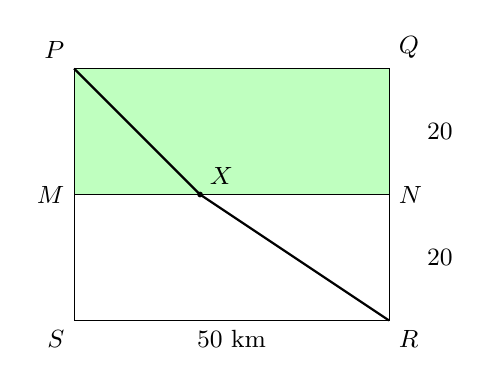
\begin{tikzpicture}[scale=.8]
  \fill[green!25] (0,4) rectangle (5,2);
  \draw (0,0) rectangle (5,4);
  \draw (0,2)--(5,2);
  \draw[thick] (0,4)--(2,2)--(5,0);
  \fill (2,2) circle (1.3pt);
  \node[above left,font=\small] at (0,4) {$P$};
  \node[above right,font=\small] at (5,4) {$Q$};
  \node[below right,font=\small] at (5,0) {$R$};
  \node[below left,font=\small] at (0,0) {$S$};
  \node[left,font=\small] at (0,2) {$M$};
  \node[right,font=\small] at (5,2) {$N$};
  \node[above right,font=\small] at (2,2) {$X$};
  \node[below,font=\small] at (2.5,0) {$50\ \mathrm{km}$};
  \node[right,font=\small] at (5.45,1) {$20$};
  \node[right,font=\small] at (5.45,3) {$20$};\end{tikzpicture}
\end{center}
\shortans{156}
\loigiai{Đặt $MX=x$ ($0\le x\le50$), $PM=20$, $MS=20$. Trong $PMNQ$: $PX=\sqrt{400+x^2}$; trong $MNRS$: $XR=\sqrt{400+(50-x)^2}$.

Thời gian (giờ): $f(x)=\dfrac{\sqrt{400+x^2}}{30}+\dfrac{\sqrt{400+(50-x)^2}}{20}$.

$f'(x)=\dfrac{x}{30\sqrt{400+x^2}}-\dfrac{50-x}{20\sqrt{400+(50-x)^2}}=0$ cho $x\approx35{,}7$, $f(35{,}7)\approx2{,}593$ giờ $\approx155{,}6\approx156$ phút.}
\end{ex}
